\documentclass[a4paper, 12pt]{paper}

\usepackage[portuges]{babel}
\usepackage[utf8]{inputenc}
\usepackage{amsmath}
\usepackage{indentfirst}
\usepackage{blindtext}
\usepackage{graphicx}
\usepackage[hyphens]{url}
\usepackage[hidelinks]{hyperref}
\usepackage{gensymb}
\usepackage[top=2cm, bottom=2cm, left=3cm, right=2cm]{geometry}
\usepackage[table]{xcolor}
\usepackage{pbox}
\usepackage{wrapfig}
\usepackage{pdflscape}

\renewcommand{\UrlFont}{\scriptsize}
\author{I. Messina, I. Abreu, P. Gil, R. Bellotti, T. Proux}

\title{Plano de Negócios - eVarsity}
\begin{document}
    \begin{titlepage}
    	\begin{minipage}[c][3cm][c]{3cm}
    		
\includegraphics[height=3cm]{img/ufrj_logo.png}
    	\end{minipage}
    	\begin{minipage}[c][3cm][c]{10cm}
    		Universidade Federal do Rio de Janeiro \\
    		Organização das Indústrias \\
    		Plano de Negócios
    	\end{minipage}
    	\begin{center}
    		\vspace{95pt}

    		\huge{Plano de Negócios - eVarsity}
    		\vspace{260pt}
    	\end{center}

    	\begin{center}
            Ian Messina \\
            Igor Abreu\\
            Pedro Gil\\
            Rafael Bellotti\\
            Thasus Proux\\
    	\end{center}

    	\begin{center}
    		\vspace{\fill}
    		Rio de Janeiro, 24 de Novembro de 2016
    	\end{center}
    \end{titlepage}
\newpage
\tableofcontents
\listoffigures
\newpage

\section{Plano de Gestão}
\subsection{Fatores Culturais}


Com os grandes avanços que ocorreram na área de tecnologia da informação nas últimas décadas, especialmente a partir da virada do milênio, os equipamentos eletrônicos estão cada vez mais presentes nos cotidianos individuais, e têm ressignificando múltiplas formas de interação entre as pessoas. As crianças nascidas neste período têm entrado em contato com computadores pessoais, consoles de videogame, tablets e smartphones cada vez mais cedo. Um dos maiores atrativos para essas gerações, ao longo de todas essas plataformas, são os jogos eletrônicos.

Por sua vez, a crescente capacidade computacional dos computadores permite a criação de jogos com complexidade crescente, apresentando desde gráficos extremamente elaborados, passando por mecânicas simplificadas de jogo através de controles por movimento, até narrativas profundas e complexas, capazes de atrair consumidores de idade mais avançada, ou interessados em elementos estéticos e literários.

Esse crescimento do escopo da produção de jogos eletrônicos, então, tem gerado um enorme crescimento dessa indústria. O mercado de jogos eletrônicos está mundialmente em ascensão e deve gerar US\$99,6 bilhões até o final do ano, se consolidando como o maior ramo da indústria do entretenimento, ultrapassando o cinema. Este valor é 8.5\% maior que o do mesmo período no ano passado. A Newzoo, empresa que realizou a pesquisa, também prevê um crescimento positivo no Brasil: considerado o décimo primeiro país com maior mercado de jogos no mundo. Além disso, os dados da pesquisa apontam que dos 33,6 milhões de usuários brasileiros, 56\% investem dinheiro em jogos.

Não é apenas através do consumo e da utilização desses jogos eletrônicos, porém, que se desenvolvem atividades. O ato de jogar se tornou, por si só, entretenimento. Jogar por diversão se tornou uma ferramenta para produção de conteúdo de distribuição online que, hoje, se consolidou como uma das maiores indústrias do entretenimento online, através de plataformas de compartilhamento de vídeo e de livestreaming como o YouTube e a Twitch. Os produtores de conteúdo focado em jogos eletrônicos representam a maior fatia de arrecadação em relação ao conjunto dos produtores independentes - os grandes canais promovidos por gigantes da mídia tradicional, como VEVO, não são aqui contabilizados.

Não é só diversão que atrai público, porém. Uma enorme indústria vem se consolidando ao longo da última década e meia, baseada em eventos que envolvem jogos eletrônicos com caráter competitivo: os esportes eletrônicos, ou eSports. Os principais títulos competitivos atuais apresentam múltiplos torneios por ano, com premiações que podem chegar à casa das dezenas de milhões de dólares\footnote{\url{http://www.pcgamer.com/dota-2-international-2016-breaks-own-prize-pool-record-now-biggest-in-esports-history/}} e com milhões de espectadores simultâneos. Empresas de mídia tradicional, apercebendo-se da tendência de crescimento da área, já se fazem presentes nesse cenário. A MTG (Modern Times Group), um conglomerado sueco de mídia e dono da ESL (Electronic Sports League) e da Dreamhack (espécie de Campus Party de proporções maiores) é um dos maiores players da indústria. A TBS (Turner Broadcast System), um dos principais canais de televisão dos EUA e propriedade da Time Warner, um dos maiores conglomerados de mídia do mundo, produz campeonatos de esportes eletrônicos para a televisão aberta norte-americana, e seu próximo evento, a ser realizado em Janeiro de 2016, apresentará 1 milhão de dólares em premiações\footnote{\url{http://www.eleague.com/major/}}. Estima-se que o número de pessoas que reconheçam os esportes eletrônicos tenha passado de 1 bilhão e que o número de espectadores tenha ultrapassado os 300 milhões\footnote{\url{https://newzoo.com/insights/articles/global-esports-awareness-exceeds-1-billion-as-new-initiatives-launched/}}.

\begin{figure}[!ht]
	\centering
	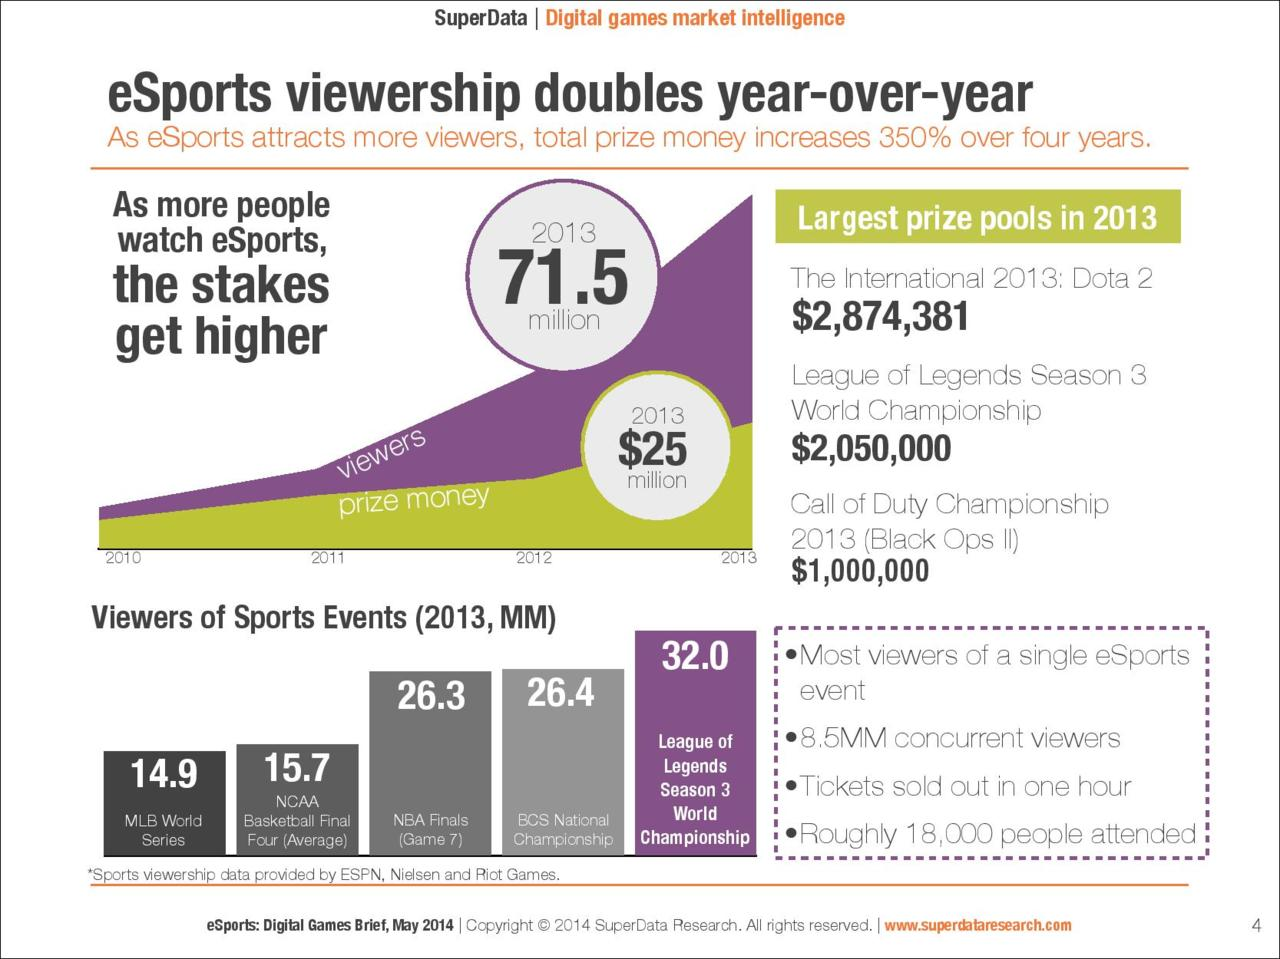
\includegraphics[scale=0.45]{img/img01.png}
	\caption{Crescimento do número de Telespectadores de eSport}
\end{figure}

Essa tendência de crescimento da audiência - e da formação de jogadores competitivos - é igualmente encontrada no Brasil, que configura na lista dos 10 países que mais assistem conteúdo deste tipo. Um dos principais times e bicampeão mundial em 2016 de um dos títulos mais assistidos de eSports, Counter-Strike:Global Offensive, é formado exclusivamente por jogadores brasileiros. O conjunto de 5 jogadores já faturarou mais de 1 milhão de dólares em premiações e, sob a organização alemã SKGaming, recebe U\$10.000,00 de salário mensal por jogador. Jogadores brasileiros de League of Legends, como Felipe “brTT” Gonçalves\footnote{\url{http://sportv.globo.com/site/games/noticia/2016/11/jogador-brasileiro-mais-famoso-de-lol-felie-brtt-deixa-pain-gaming.html}} e Gabriel “Kami” Bohn\footnote{\url{http://sportv.globo.com/sit e/games/noticia/2016/07/gabriel-kami-o-jovem-fenomeno-do-lol-no-brasil-que-vale-r-1-milhao.html}}, por suas vezes, figuram entre os 10 jogadores de eSports com maior número de seguidores no mundo.

\begin{figure}[!ht]
	\centering
	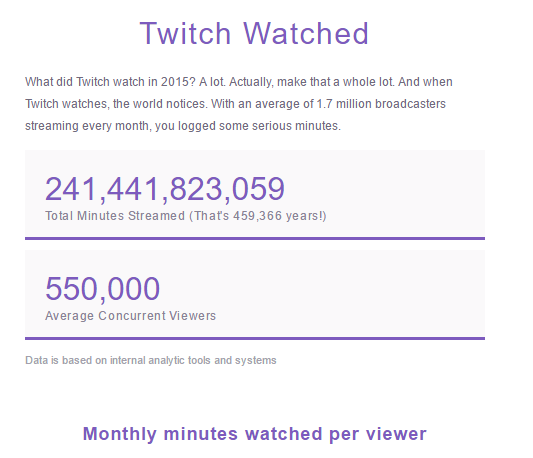
\includegraphics[scale=1]{img/img02.png}
	\caption{Dados sobre a plataforma de Streaming da Twitch}
\end{figure}
É possível afirmar que existe, então, um mercado consumidor bastante significativo no Brasil, tanto de jogadores quanto de espectadores de esportes eletrônicos. Um mercado, porém, ainda muito pouco explorado. A grande maioria dos eventos e produtoras internacionais de real importância quase nunca puseram os pés no país, relegando torneios de nível mais baixo para aqui serem sediados. Também, o cenário nacional de eSports se mostra bastante amador e incipiente, ainda. Os produtores locais, assim como as organizações de jogadores e os times nacionais que não se mudaram para outros continentes, possuem pouca influência internacional e pequenas capitalizações. O cenário local de eSports é praticamente intocado por grandes empreendimentos, ou mesmo por empreendimentos de caráter verdadeiramente profissional. Em suma, o mercado de eSports no Brasil é fértil e pouquíssimo explorado.
\subsection{Fatores Ambientais}
Os eventos serão separados em etapas online e presenciais. As etapas online não apresentam diretamente nenhum impacto ambiental, pois seu conteúdo está atrelado ao meio virtual. Os eventos presenciais apresentam risco de poluição sonora; porém, poderiam ser sediados em lugares propriamente aparelhados com proteção acústica projetada, podendo abaixar esse risco até que seja considerado nulo.
\subsection{Fatores Mercadológicos}
Três tipos de consumidor devem ser levados em conta. É considerado um consumidor em potencial do primeiro tipo todos que possuem um computador conectado à rede e que tenham interesse por jogos eletrônicos e estejam interessados em participar ou assistir os jogos. Os consumidores do segundo tipo são clientes que desejam contratar serviços de consultoria para ajudar a planejar eventos de jogos competitivos. Os do terceiro tipo são empresas que busquem oferecer patrocínio a eventos de esportes eletrônicos em troca da divulga\c{c}\~{a}o de suas marcas e de outros \textit{payoffs}. A seguir será realizado uma análise dos principais agentes no mercado de jogos eletrônicos.
\subsubsection{Serviços de Streaming}
Serviços de streaming como YouTube e Twitch influenciam fortemente o mercado de jogos. Por se tratar das plataformas de acompanhamento de jogos em tempo real mais fortes no mercado, se torna indispensável considerar seus efeitos no mercado de jogos.

De acordo com a plataforma Twitch, a média de espectadores simultâneos é de 550 mil e o número de minutos médios que cada espectador assiste usando a plataforma Twitch é de 421,6 por mês, já na plataforma YouTube foram 291 minutos por mês. O gráfico abaixo mostra o crescimento do número de espectadores e canais entre dia 20 de junho de 2012 e dia 29 de outubro de 2016 na plataforma Twitch.
\begin{figure}[!ht]
	\centering
	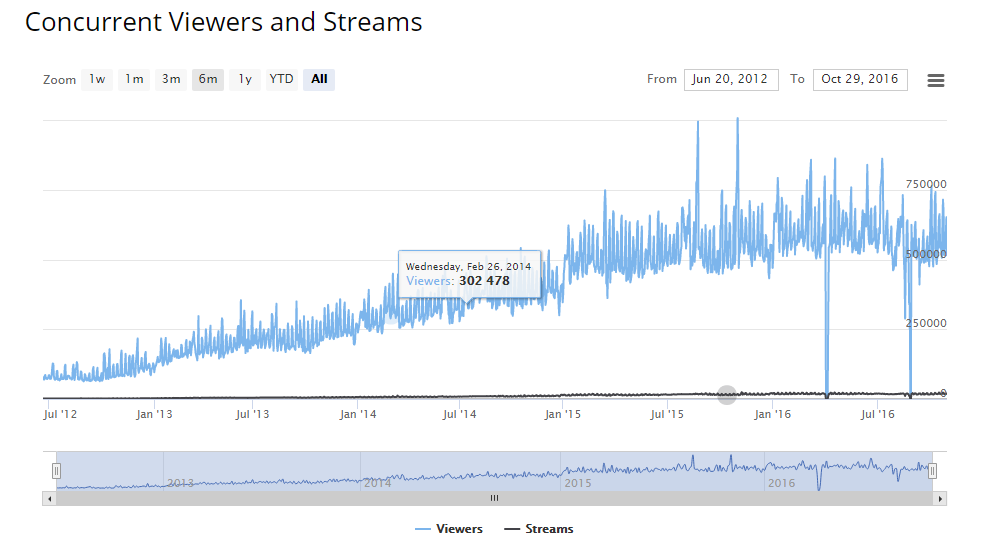
\includegraphics[scale=0.62]{img/img03.png}
	\caption{Aumento do número de telespectadores na plataforma de Streaming da Twitch}
\end{figure}
\subsubsection{Eventos Presenciais}
Eventos de competição presenciais reúnem espectadores e competidores em um único espaço, onde os primeiros têm a oportunidade de observar os jogadores competindo. As empresas que criam os jogos tendem a dar reconhecimento a tais eventos e costumam ajudar na divulgação deles em suas páginas web e nas áreas de notícias dentro do portal de seus jogos.

Para exemplificar com números, o IEM Katowice, realizado em Fevereiro de 2016, teve mais de 104 mil espectadores somente no evento, ou seja, sem contar com os espectadores que assistiam por meio da televisão ou plataformas de streaming.

O The International 2016, maior campeonato de Dota 2 do ano, que teve mais de 17 mil pessoas simultaneamente em um estádio, chegou a uma premiação de U\$20.770.460, o meio valor de premiação da história dos eSports - e maior do que a premiação de alguns dos maiores eventos esportivos do mundo, como o Superbowl \footnote{\url{http://www.polygon.com/2014/7/19/5918845/dota-2-international-2014-champions-money-winners}}. Desse valor, somente U\$1.600.000,00 vieram da empresa Valve, criadora do jogo e responsável pela organização do evento; todo o resto foi obtido via ferramentas de financiamento coletivo, direto dos espectadores do evento.
\subsubsection{Televisão}
Embora ainda tenham pouco impacto no mundo da transmissão por televisão, os eSports estão crescendo nesse tipo de mídia. Atualmente, canais de grande nome, como CNN, TBS e ESPN, no caso internacional, e SporTV e Esporte Interativo no caso nacional, estão cada vez mais investindo em jogos eletrônicos para atrair mais espectadores para seus canais de televisão\footnote{\url{http://esporteinterativo.com.br/esports/eleague-chega-aos-canais-esporte-interativo-e-reacende-a-paixao-do-brasil-por-counter-strike/}}\footnote{\url{http://sportv.globo.com/site/noticia/2016/04/sportv-inova-e-transmite-ao-vivo-torneio-do-game-dota-2.html}}. Além disso, a empresa ESL anunciou um canal de televisão dedicado a jogos eletrônicos chamado de esportsTV.
\subsection{Fatores Geográficos}
Os eventos puramente online não apresentam nenhuma barreira geográfica, mas são passíveis de gerar barreiras para usuários de regiões com acesso limitado à internet. Por outro lado, os eventos presenciais requerem que os espectadores estejam no evento fisicamente. Isto acaba gerando uma forte barreira geográfica, pois somente pessoas nativas ao local de realização do evento, ou com condições financeiras favoráveis para bancar os custos de viagens, hospedagem e do evento em si, além de possuírem tempo disponível, poderão participar dos eventos.
\subsection{Fatores Econômicos}
A economia do país está apresentando resultados surpreendentes com os poucos eventos que foram organizados. São Paulo sediou nos dias 28 a 30 de outubro de 2016 a quarta edição do torneio de CS:GO Pro League, premiando o primeiro colocado com US\$200.000, sendo as premiações totais somadas equivalentes a US\$750.000. O Ginásio do Ibirapuera foi completamente  tomado, com todos os ingressos, para todos os dias do evento, tendo sido vendidos. A audiência online ultrapassou 100.000 espectadores simultâneos nos momentos de pico.

Outro grande fator é o crescimento do poder de compra da população brasileira em relação ao período inicial de desenvolvimento dos eSports, há mais de uma década atrás. Mesmo com os impactos do presente momento de instabilidade econômica pelo qual passa o país, é possível afirmar que a disponibilidade de renda média da população brasileira para consumo de jogos eletrônicos - e, indiretamente, de produtos ligados aos eSports - é maior. Junte-se a isso o fato de que os preços dos jogos estão cada vez mais acessíveis, por conta do advento da distribuição digital, que reduz os custos de distribuição ao fornecer o download direto dos jogos via internet, e é possível afirmar que existe um grande potencial econômico para o desenvolvimento deste cenário.

Deve-se também levar em conta que as plataformas de transmissão por meio digital são abertas de forma gratuita a qualquer um que tenha acesso a internet. Dessa forma, qualquer um que possa acessar os sites pode acompanhar os jogos e campeonatos, de forma que a barreira de entrada para espectadores é muito pequena.
\subsection{Fatores Sociais}
Uma grande parcela dos interessados nessas modalidades são jovens-adultos - muitos universitários - e adolescentes, embora a demografia esteja se expandindo em ambas as direções do espectro. É considerado de vital importância, então,  não somente planejar eventos pensando nos calendários acadêmicos, como também oferecer opções baratas de pacotes que cubram menos atividades durante o evento, mas que permitam a jovens com recursos financeiros limitados assistirem aos jogos.
\subsection{Fatores Tecnológicos}
O projeto é inteiramente baseado em tecnologia. Tanto os eventos presenciais quanto os online são construídos em cima de competições realizadas em computadores e via infraestrutura de rede e hospedagem de servidores. Não apenas a competição em si, porém, mas também todo o mecanismo de cobertura e de transmissão das partidas, tanto \textit{in loco} quanto via internet, são realizados através de meios digitais.

Para realização de eventos online, é necessária infraestrutura remota de hospedagem em servidores para a conexão dos jogadores à partida e um sistema para observação e transmissão do jogo via livestream, assim como mecanismos de pós-produção para realizar as transições entre as diferentes telas (composição dos times, estatísticas, etc.).


\begin{wrapfigure}{l}{5.5cm}
    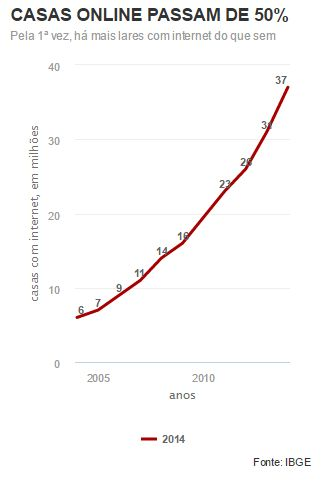
\includegraphics[scale=0.5]{img/img04.png}
    \caption{Casas com acesso \`{a} internet}
\end{wrapfigure}

Para realização de eventos \textit{in loco}, é necessária infraestrutura presencial de hospedagem de servidores próprios para conexão dos jogadores à partida e o mesmo sistema para observação e transmissão, também com pós-produção. Neste caso, além da pós-produção do conteúdo diretamente relacionado ao jogo, existe a possibilidade da existência de câmeras filmando o evento em tempo real, o que implica na necessidade de produção e filtragem de canais simultâneos de imagens ao vivo, assim como de iluminação e estudo de captação de áudio.
No campo da produção posterior de conteúdo em cima dos eventos, é necessária estrutura para captura de vídeo e de som direto dos jogos, em alta definição e fidelidade, assim como para captação de vídeos do ambiente do evento em alta qualidade, com boa iluminação e captação de som.

Excedendo-se o caráter da produção e direcionando o foco para o consumo,disso, é fundamental que o espectador que não esteja \textit{in loco} possua acesso à internet. O IBGE publicou, através da PNAD de 2011, dados que mostram que o acesso a internet cresceu para todas as camadas sociais do país. Isto se deve, provavelmente, a melhorias no mercado de trabalho e na renda pessoal, além de expansão da área de cobertura e melhoria da infraestrutura existente, o que implicou na redução de custos para contratação deste tipo de serviço.

Os dados do IBGE referentes a 2014 mostram que 36,8 milhões de domicílios estavam conectadas à internet, representando um total de 54,9\% da população brasileira. Tal índice é consideravelmente maior que o de 2013 (48\%), mostrando crescimento considerável desse segmento.

Além disso, o IBGE indicou que a quantidade de internautas chegou a 54,4\% das pessoas com mais de 10 anos em 2014. São 95,4 milhões de brasileiros com acesso a internet. Essa dupla ultrapassagem vem de uma mudança de metodologia do IBGE. Apenas as conexões feitas com computador eram registradas até a PNAD de 2013; a partir daí, o instituto passou a contabilizar acessos com smartphones, tablets, TVs e outros dispositivos, todos passíveis de ser utilizados como meios de acompanhar o cenário competitivo de esportes eletrônicos.

Além disso, de acordo com dados da Wikipedia, de 2012, o Brasil atualmente se encontra em quarto no ranking dos países que possuem o maior número absoluto de pessoas com acesso a internet.

\begin{figure}[!ht]
    \centering
    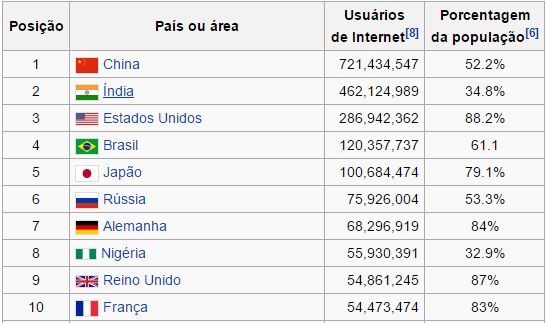
\includegraphics[scale=0.5]{img/img05.png}
    \caption{Us\'{u}arios de internet por pa\'{i}ses}
\end{figure}

\newpage

\begin{landscape}
\subsection{Análise SWOT}
    \begin{figure}[!ht]
        \centering
        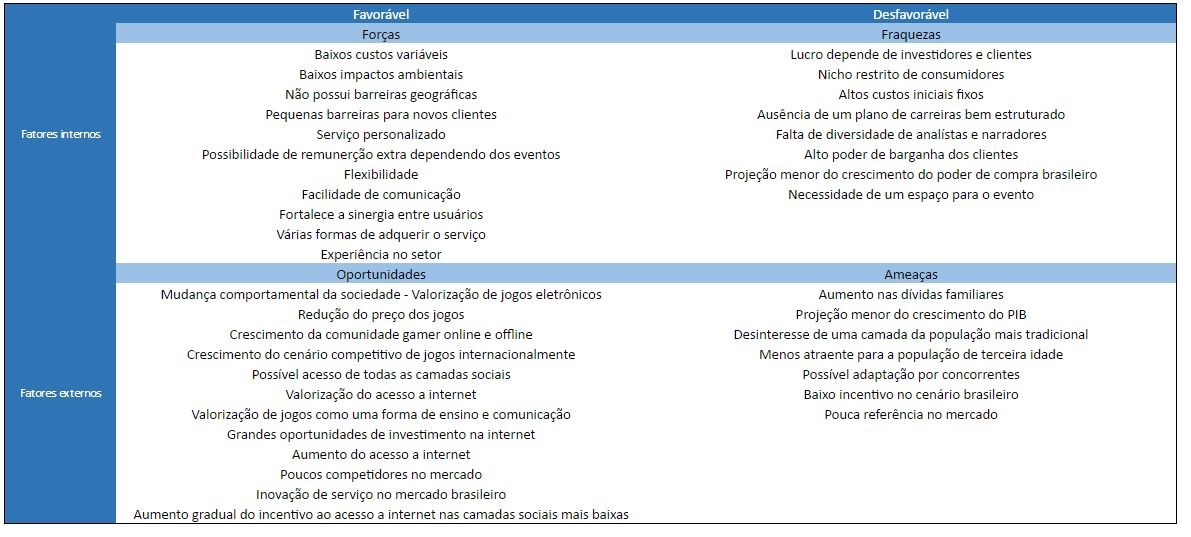
\includegraphics[width=25cm,height=12cm]{img/img06.png}
        \caption{Análise SWOT}
    \end{figure}
\newpage
\subsection{Modelo de Negócio Canvas}
\begin{figure}[!ht]
    \centering
    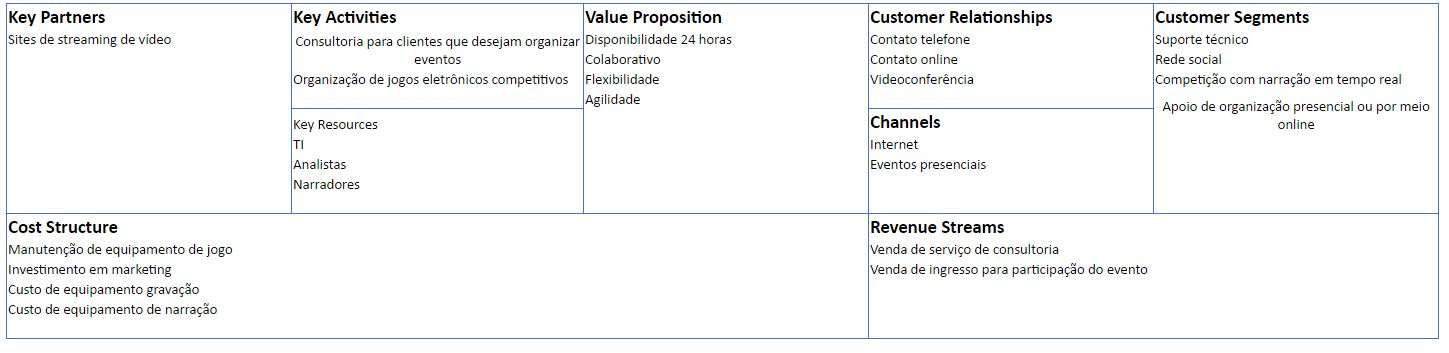
\includegraphics[width=25cm,height=10cm]{img/img07.png}
    \caption{Modelo Canvas}
\end{figure}
\newpage
\subsection{Fatores Críticos de sucesso}
\begin{figure}[!ht]
    \centering
    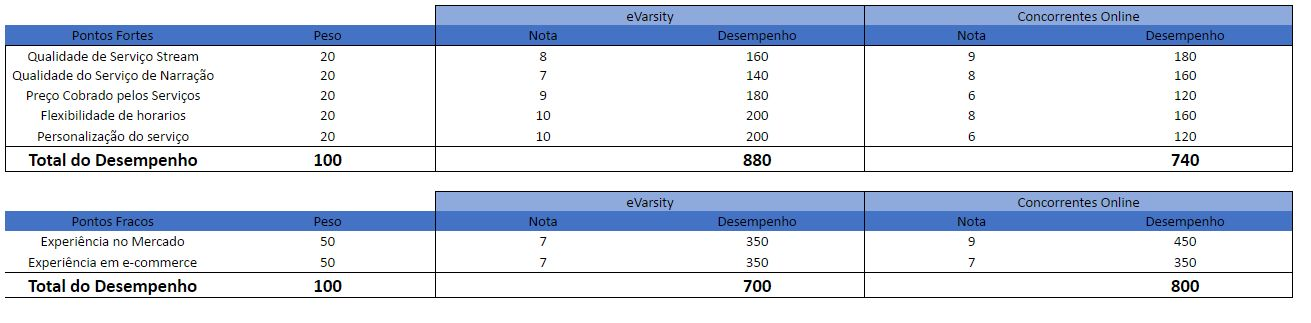
\includegraphics[scale=0.56]{img/img08.png}
    \caption{Posicionamento Competitivo}
\end{figure}
Ao examinar o posicionamento competitivo da eVarsity, ao interpretar os números encontrados na análise dos pontos fortes da empresa, é fácil perceber o diferencial da empresa em relação aos concorrentes.  Porém, em relação aos pontos fracos, existe clara desvantagem no que se refere aos possíveis concorrentes. Isso, porém, é apenas uma maneira de ilustrar a divisão clara entre o nicho de mercado a ser afetado pela eVarsity, composto principalmente pelo cenário amador/semi-profissional Universitário e acadêmico, e o nicho focal de seus concorrentes, composto pelo cenário “profissional”. A eVarsity, embora possua concorrentes gerais, não possui nenhum concorrente direto. Mesmo que afetando um mesmo mercado geral, os nichos específicos não se mostram concorrentes.
\end{landscape}



\newpage
\section{Plano de Marketing}
\subsection{Descrição dos Serviços}
\subsection{Forças do Marketing}
\subsubsection{Produto}
\subsubsection{Preço}
\subsubsection{Praça}
\subsubsection{Promoção}
\subsubsection{Pessoas}
\subsubsection{Processos}
\newpage
\section{Plano Operacional}
\subsection{Layout Operacional}
\subsection{Capacidade de Prestação}
\subsection{Processos Operacionais}
\subsection{Necessidade inicial de colaboradores}
\newpage
\section{Plano Financeiro}
\subsection{Investimentos Iniciais}
\subsection{Capital de Giro}
\subsection{Investimentos Pré-Operacionais}
\subsection{Investimento Total}
\subsection{Estimativa de faturamento}
\subsection{Estimativa do custo de comercialização}
\subsection{Estimativa do custo de cada produto vendido}
\subsection{Custos com Depreciação}
\subsection{Custos Operacionais}
\subsection{DRE}
\subsection{O Fluxo de Caixa}
\subsection{Indicadores de Viabilidade}
\subsection{Cenário Alternativo}
\newpage
\section{Estrutura da Empresa}
\subsection{Estrutura Organizacional}
\subsection{Estrutura jurídica}

\end{document}